\documentclass{article}
\usepackage[utf8]{inputenc}
\usepackage{polski}
\usepackage{graphicx}
\graphicspath{{images/}}
\usepackage{url}
\usepackage{dirtytalk}
\usepackage{booktabs}
\usepackage{float}
\usepackage{caption}
\usepackage{subcaption}

\usepackage{geometry}
\newgeometry{tmargin=4cm, bmargin=4cm, lmargin=3.2cm, rmargin=3.2cm} 


\begin{document}


\begin{titlepage}

\begin{center}

    \LARGE \textsc{Politechnika Wrocławska}\\
    \vspace*{0.2cm}
    \Large \textsc{Wydział Informatyki i Telekomunikacji}\\  
    \vspace*{0.4cm}
    \centering\includegraphics[width=0.2\textwidth]{WITlogo.png}\\
    \vspace*{0.2cm}
    \vspace*{2cm}

    \centerline{\rule{\textwidth}{1.2pt}}
    \vspace{0.4cm}
    \Huge\textbf{Sieci złożone}
    \centerline{\rule{\textwidth}{1.2pt}}
    \vspace{1cm}
    \LARGE Sprawozdanie z laboratorium\\
    \vspace{2.7cm}

    \textsc{Autor}\\
    \vspace{0.2cm}
    \textbf{Jędrzej Jamnicki}\\
    \vspace{0.1cm}
    \Large nr albumu: \textbf{254290}\\
    \vspace{0.2cm}
    kierunek: \textbf{Inżynieria systemów}

    specjalizacja: \textbf{Inżynieria danych}

    \vspace{1.35cm}
    \Large \textit{28 stycznia 2022}

\end{center}

\end{titlepage}

\begin{abstract}
Celem badań jest analiza słownictwa użytego w artykułach z wielojęzycznej encyklopedii internetowej - \textit{Wikipedia} w oparciu o zbiór 4,604 artykułów spośród 15 kategorii.
\end{abstract}

\section{Wstęp}

Dane zostały pobrane z \url{https://snap.stanford.edu/data/wikispeedia.html} w formie plików w formacie \textit{txt} wraz z przypisanymi im kategoriami takimi jak matematyka, sztuka czy historia.

Artykuły w \say{surowej} formie nie mogą zostać poddane analizie. Muszą zostać poddane wstępnemu przetwarzaniu czyli swojego rodzaju oczyszczenia tekstu z m.in. takich szumów jak znaki specjalne (czasami są pożądane) Następnym etapem jest wyznaczenie unikalnego zbioru słów w formie podstawowej (hasłowej) zwanych dalej \textit{tokenami} oraz określenie ich część mowy dla każdej z danych kategorii.

Do przetwarzania zbioru danych użyto języka programowania \texttt{Python}, wizualizacje przedstawiono przy
użyciu biblioteki \texttt{altair}.

\section{Analiza}

Artykuły poddano wstępnemu przetwarzaniu, kolejno:
\begin{itemize}
    \item usunięto znaki specjalne oraz cyfry
    \item usunięto zduplikowane białe znaki
    \item usunięto słowa o długości mniejszej niż 3 znaki
    \item usunięto słowa wchodzące w skład tzw. stop listy
    \item sprowadzono litery do jednolitego formatu (małych liter)
    \item sprowadzono słowa do formy podstawowej (lematyzacja)
\end{itemize}

Do wyeliminowania niechcianych znaków w tekście użyto wyrażeń regularnych.
Do lematyzacji oraz usunięcia słów ze stop listy wykorzystano bibliotekę \texttt{nltk} (korpus WordNet)
\vspace{0.5cm}

Zliczono wystąpienia tokenów dla każdej kategorii. Z wykorzystaniem metody \texttt{nltk.pos\_tag} określono
część mowy (\textit{Part-of-Speech}) dla każdego z nich. Na podstawie ilości wystąpień oraz sumarycznej ilości unikalnych tokenów we wszystkich artykułach dla poszczególnej kategorii wyznaczono częstotliwości występowania.

\newpage
Otrzymane wartości zapisano do ramki danych biblioteki \texttt{Pandas} prezentującej się następująco:

\begin{table}[H]
    \centering
        \begin{tabular}{lllrr}
            \toprule
            Category &      Token & Part-of-Speech &  Occurrences &  Frequency \\
            \midrule
               History &         klan &                  Noun &          188 &   0.001222 \\
               History &         hmas &                Adverb &          131 &   0.000851 \\
               History &      titanic &             Adjective &          108 &   0.000702 \\
               History &      seacole &                  Verb &           98 &   0.000637 \\
               History &   yugoslavia &                Adverb &           86 &   0.000559 \\
               History &      colditz &                  Noun &           77 &   0.000500 \\
                \vdots &       \vdots &                \vdots &       \vdots & 	   \vdots \\
             Countries &       celtic &                  Noun &            8 &   0.000101 \\
             Countries &      galicia &             Adjective &            8 &   0.000101 \\
             Countries &   zimbabwean &                  Noun &            5 &   0.000063 \\
             Countries &      lankans &                  Verb &            5 &   0.000063 \\
            \bottomrule
        \end{tabular}\\
        1322306 rows × 5 columns
        \vspace{0.25cm}
        \caption{Dane każdego z tokenów.}
        \label{tab:tokens_table}
\end{table}

Związek tokenów z kategoriami przedstawiono również w postaci grafu dwudzielnego,
w którym zbiór górnych wierzchołków stanowią tokeny a dolnych - kategorie.

\begin{figure}[H]
    \begin{center}
        \makebox[0pt]{\includegraphics[width=17cm]{bipartite_graph.png}}
        \caption{Graf dwudzielny reprezentujący zbiór danych.}
        \label{fig:bipartite_graph}
    \end{center}
\end{figure}

\begin{table}[H]
    \centering
        \begin{tabular}{lrr}
            \toprule
                           Category &  Tokens &  Files \\
            \midrule
                          Geography &  220024 &   1084 \\
                             People &  184725 &    689 \\
                            Science &  154367 &   1122 \\
                            History &  153855 &    545 \\
                      Everyday\_life &  100361 &    374 \\
                          Countries &   79565 &    229 \\
            Language\_and\_literature &   65750 &    196 \\
              Design\_and\_Technology &   63841 &    254 \\
                        Citizenship &   62802 &    224 \\
                           Religion &   54071 &    134 \\
                              Music &   38039 &     97 \\
                   Business\_Studies &   29105 &     88 \\
                                 IT &   28624 &     85 \\
                                Art &   16890 &     38 \\
                        Mathematics &   13486 &     45 \\
            \bottomrule
        \end{tabular}
        \vspace{0.25cm}
        \caption{Ilość unikalnych tokenów oraz plików dla kategorii.}
        \label{tab:categories_table}
\end{table}


\begin{figure}[H]
    \begin{center}
        \makebox[0pt]{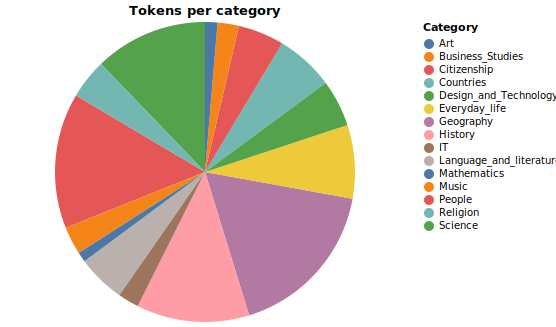
\includegraphics[width=12cm]{charts/tok_per_cat.png}}
        \caption{Ilość unikalnych tokenów dla każdej z kategorii.}
        \label{fig:tok_per_cat}
    \end{center}
\end{figure}

\begin{figure}[H]
    \begin{center}
        \makebox[0pt]{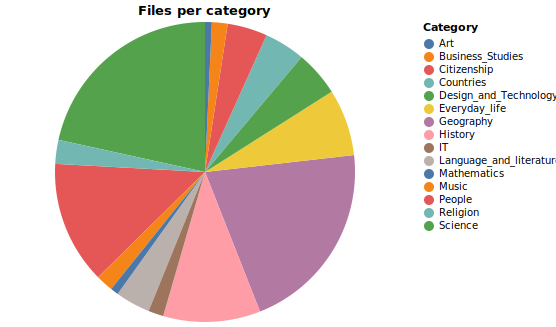
\includegraphics[width=12cm]{charts/files_per_cat.png}}
        \caption{Ilość artykułów dla każdej z kategorii.}
        \label{fig:files_per_cat}
    \end{center}
\end{figure}

Tab. \ref{tab:categories_table} oraz rys. \ref{fig:tok_per_cat}, \ref{fig:files_per_cat} pokazują,
że każda z kategorii reprezentuje nieproporcjonalną część zbioru danych, co nie napawa optymizmem
przed kolejnymi analizami.

Na podstawie wartości z tab. \ref{tab:tokens_table} wyznaczono procentowy udział części mowy
dla każdej kategorii.

\begin{table}[H]
    \centering
        \begin{tabular}{lllll}
            \toprule
                           Category &   Noun & Adjective & \ldots & Adverb \\
            \midrule
                          Geography & 0.5965 &    0.2371 & \ldots & 0.0411 \\
                             People & 0.5716 &    0.2335 & \ldots & 0.0472 \\
                            Science & 0.5803 &    0.2304 & \ldots & 0.0479 \\
                            History & 0.5627 &    0.2445 & \ldots & 0.0458 \\
                     Everyday\_life & 0.5817 &    0.2240 & \ldots & 0.0464 \\
                          Countries & 0.5961 &    0.2405 & \ldots & 0.0401 \\
          Language\_and\_literature & 0.5881 &    0.2340 & \ldots & 0.0481 \\
            Design\_and\_Technology & 0.5792 &    0.2217 & \ldots & 0.0471 \\
                        Citizenship & 0.5555 &    0.2473 & \ldots & 0.0439 \\
                           Religion & 0.5685 &    0.2439 & \ldots & 0.0469 \\
                              Music & 0.5713 &    0.2312 & \ldots & 0.0522 \\
                  Business\_Studies & 0.5633 &    0.2339 & \ldots & 0.0469 \\
                                 IT & 0.5591 &    0.2260 & \ldots & 0.0523 \\
                                Art & 0.5571 &    0.2385 & \ldots & 0.0504 \\
                        Mathematics & 0.5708 &    0.2354 & \ldots & 0.0529 \\
            \bottomrule
        \end{tabular}
        \caption{Procentowy udział części mowy według kategorii.}
        \label{tab:categories_pos_ratio}
\end{table}


Diagramy kołowe stworzone dla każdej kategorii pokazały, że nie odbiegają od siebie nawzajem pod względem
procentowego udziału części mowy w artykułach. Diagramy dla dwóch kategorii przedstawiono poniżej:

\begin{figure}[H]
    \centering
    \begin{subfigure}{.38\textwidth}
        \centering
        \makebox[0pt]{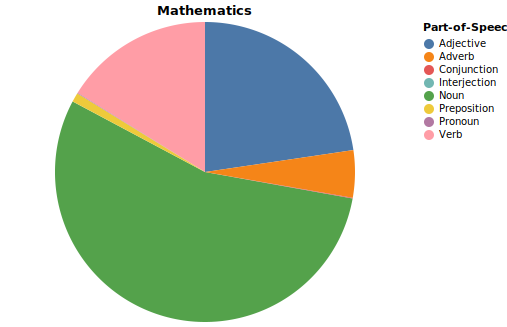
\includegraphics[width=9cm]{charts/math_pos.png}}
        \caption{Matematyka}
        \label{fig:math_pos}
    \end{subfigure}%
    \begin{subfigure}{.6\textwidth}
        \centering
        \makebox[0pt]{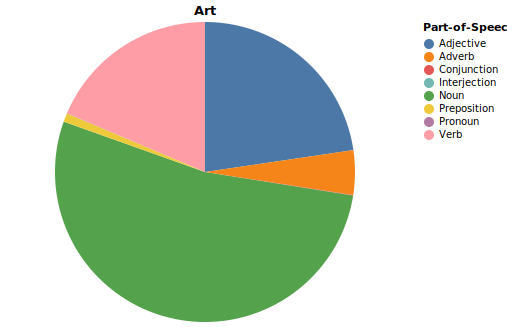
\includegraphics[width=9cm]{charts/art_pos.png}}
        \caption{Sztuka}
        \label{fig:art_pos}
    \end{subfigure}
    \caption{Procentowy udział części mowy dla kategorii.}
    \label{fig:duo_cat_pos}
\end{figure}

Na zakończenie zbadano ilość wspólnych tokenów między kategoriami. W tym celu stworzono macierz, w której
każdy element odpowiada procentowej wartości tokenów wspólnych. Do wizualizacji wykorzystano diagram korelacji przedstawiony na rys. \ref{fig:common_tokens} poniżej.

\begin{figure}[H]
    \centering
    \makebox[0pt]{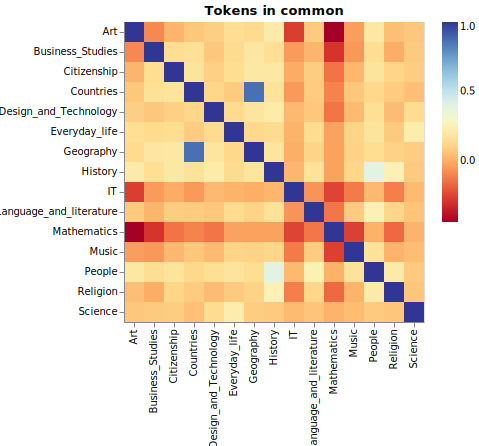
\includegraphics[width=10cm]{charts/tok_cat_corr.png}}
    \caption{Procentowa wartość wspólnych tokenów między kategoriami.}
    \label{fig:common_tokens}
\end{figure}

\section{Wnioski}

Tab. \ref{tab:categories_pos_ratio} oraz rys. \ref{fig:math_pos}, \ref{fig:art_pos} jasno pokazują, że części mowy są ściśle między sobą powiązane i nie odbiegają procentowym udziałem w artykułach
między kategoriami. 

\paragraph{}
Na rys. \ref{fig:common_tokens} zauważono silną korelację między kategoriami:
\begin{itemize}
    \item Geografia - Kraje (aż ~86.62\%)
    \item Ludzie - Historia (aż ~39.41\%)
    \item IT -- Sztuka (jedynie ~28.36\%)
    \item Matematyka - Sztuka (jedynie ~19.90\%)
\end{itemize}

Części wspólne lub przeciwstawne wydają się być logiczne. Ponadto Historia wykazuję się wysoką średnią wartością wspólnych tokenów między wszystkimi innymi kategoriami, bo aż ~38.31\%. W końcu historia to
\say{wszystko w przeszłości}\ldots

\end{document}
